%!TEX root = ../main.tex

\chapter{Methodology\label{chap:methodology}}

\section{Comparison of event-based and frame-based cameras}

Traditional frame-based (either rolling or global shutter) cameras capture the scene as a sequence of still image frames at fixed intervals with fixed settings, providing a synchronous representation of the visual world. 
In terms of ease of use and the simplicity of the post-processing of data obtained from such cameras, they are wildly applicable across many fields.
A single frame obtained from a frame-based camera may be described by the following equation \refeq{eq:frame}~\cite{scheerlinck2018event}
\begin{equation}
Y_j(\boldsymbol{p}) := \frac{1}{\epsilon} \int_{t_j - \epsilon}^{t_j} Y(\boldsymbol{p}, \tau) \mathrm{d} \tau, \quad j \in 1, 2, 3 ...
\label{eq:frame}
\end{equation}
where $Y(\boldsymbol{p}, t)$ denotes the irradiation intensity of a camera pixel at a specific time $t$, $t_j$ is the time-stamp of the image capture and $\epsilon$ is the exposure time.
As can be seen, each frame is represented by a temporal average of irradiance over the exposure time $\epsilon$. Although this model simplifies image formation, it introduces artifacts such as motion blur, particularly when fast-moving objects are captured with an exposure time mismatched to their dynamics.

\ac{DVS} (or event-based cameras), are vision sensors that draw their inspiration from biological receptors in the retina of the eye, where each pixel reacts
to change of the illumination in the scene. Each pixel individually recognizes a logarithm of the intensity and compares it to the previously
recorded value. When a predefined threshold is crossed, this value is reset to the current one and a new event is generated. This event can be expressed as $e = \begin{bmatrix} x & y & \sigma & t \end{bmatrix}$, where $\begin{bmatrix} x & y \end{bmatrix}$
is the camera pixel coordinate, $\sigma$ is the polarity of change (where $\sigma = \pm 1$ for increasing or decreasing change, respectively) and $t$ is the timestamp of the event~\cite{gallego22event}~\cite{scheerlinck2018event}. The single event can be modeled as a Dirac delta function $\delta(t)$
and an event stream
$e_i(\boldsymbol{p}, t)$ can be defined at a pixel $\boldsymbol{p}$ by \refeq{eq:event_eq}~\cite{scheerlinck2018event},
with the threshold for generating an event described by the equation \refeq{eq:bias_eq}.
\begin{equation}
e_i(\boldsymbol{p}, t) := \sigma_i^{\boldsymbol{p}} c \, \delta(t - t_i^{\boldsymbol{p}}), \ i \in 1, 2, 3 ...
\label{eq:event_eq}
\end{equation}
\begin{equation}
\sigma_i^{\boldsymbol{p}} c = \log(Y(\boldsymbol{p}, t_i)) - \log(Y(\boldsymbol{p}, t_{i-1}))
\label{eq:bias_eq}
\end{equation}
where $\sigma_i^{\boldsymbol{p}}$ is the polarity (sometimes referred simply as an ON or OFF event) and $t_i^{\boldsymbol{p}}$ is the timestamp of the $i$-th event at a pixel.
The magnitude $c$ is the contrast threshold, a preset constant that defines a change in light intensity that is encoded by a singular event, at each pixel. Event-based cameras thus circumvent many common issues found in traditional frame-based cameras, such as the motion blur mentioned before. They offer significant advantages, including high dynamic range, low latency,
and energy efficiency.
This makes them perfect for the application of agile robotics,
where the fast response time is crucial (especially in UAV swarming situations). With their submillisecond response time,
event-based cameras can provide a significant advantage over traditional cameras in these applications.
However, they also come with some drawbacks, such as the need for a different approach to
data processing. While it is possible to reconstruct a logarithmic image from the event stream through temporal integration,
enabling the use of conventional vision algorithms, this approach fundamentally undermines the core advantages of event-based cameras.
The higher cost of the camera units themselves can also be the deciding factor.~\cite{gallego22event}

During recording, many camera settings can be changed, such as the \ac{ROI} settings and the bias settings.
The \ac{ROI} setting during recording takes a rectangular region in pixel coordinates and discards events outside the specified region at the hardware level, while reducing computational load and noise from irrelevant areas. This setting is especially useful in cases where only a small static area needs to be observed or where many unrelated events
may be generated, which would interfere with the measurement process.

The bias settings are a global camera setting parameters analogous to ISO or exposure time in traditional cameras, though they operate on fundamentally
different principles.
The configurable biases for the \texttt{EVK4} which directly influence event generation and noise filtering, are as follows~\cite{dilmaghani2022controlevaluationeventcameras}
\begin{itemize}
    \item \texttt{bias\_diff\_on} adjusts the threshold on which events are generated; with higher setting, the more increasing change in pixel brightness needs to be present to trigger a generation of an event with positive $\sigma$
    \item \texttt{bias\_diff\_off} adjusts the threshold on which events are generated; with higher setting, the more decreasing change in pixel brightness needs to be present to trigger a generation of an event with negative $\sigma$
    \item \texttt{bias\_fo} adjusts the low-pass filter which filters out the fast fluctuations in light intensity, effectively setting the maximum detectable oscillation frequency
    \item \texttt{bias\_hpf} adjusts the high-pass filter which filters out the slow fluctuations in light intensity, setting the minimum detectable oscillation frequency
    \item \texttt{bias\_refr} adjusts the pixel refractory period in which a pixel is inactive after generating an event
\end{itemize}
These settings were optimized during data acquisition to suppress noise and extraneous events (such as from wall reflections or scene illumination changes), which
ensured that only events related to the experiment were captured.

% =========== CALIBRATION =============

\section{Fisheye calibration model}

To ensure accurate representation of distances and angles in the output data of the camera, a calibration needs to be performed with the specific lenses
that are used. In this thesis a calibration method proposed by Scaramuzza et al.~\cite{scaramuzzacalibration} for omnidirectional camera
calibration is used to calibrate all the equipment used. 
After the calibration is performed, a mapping of the 3D world coordinates to the 2D image plane is able to be calculated.
For this, the calibration method needs to obtain the extrinsic
and intrinsic parameters of the camera, where the extrinsic parameters are the rotation and translation of the camera with respect to the world frame and can be expressed by equation \ref{eq:extrinsic},
\begin{equation}
	\begin{bmatrix}
		X_{camera} \\
		Y_{camera} \\
		Z_{camera}
	\end{bmatrix}
	= \mathbf{R} 
  \begin{bmatrix}
	X_{world} \\
	Y_{world} \\
	Z_{world}
  \end{bmatrix}
  + \mathbf{t}
  \label{eq:extrinsic}
\end{equation}
which is an affine transformation that uses a rotation matrix $\mathbf{R} \in \text{SO}(3)$ and a translation vector
$\mathbf{t} \in \mathbb{R}^3$. The origin of the camera's coordinate system is at the optical center,
that is, at the intersection of the optical axis from the center of the image with the image plane. This can be represented by \reffig{fig:camera_extrinsic}.

\begin{figure}[H]
  \centering
  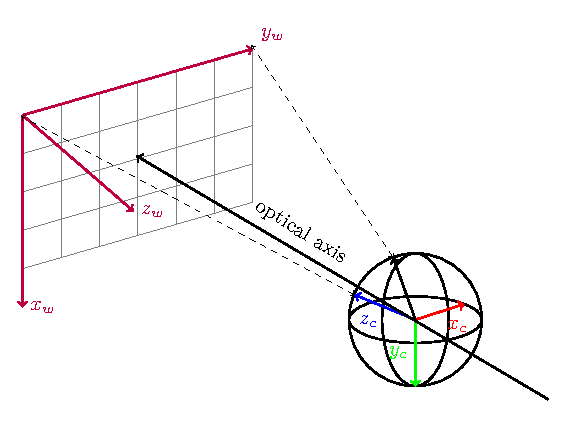
\includegraphics[width=0.7\textwidth]{./fig/tikz/extrinsic.pdf}
  \caption{Extrinsic parameters of the camera~\cite{scaramuzzacalibration}.}
  \label{fig:camera_extrinsic}
\end{figure}

The next step in the camera calibration is to fit an encompassing ellipse to the received data. The purpose of this is to see the center of distortion of the fisheye lens, as well
as the stretching of the image on both the x and y axes. This process can be seen in \reffig{fig:ellipse}. This ellipse is then used to calculate the point-mapping functions, which allows for transformation of points from
the image plane to their respective 3D coordinates.
\begin{figure}[H]
	\centering
	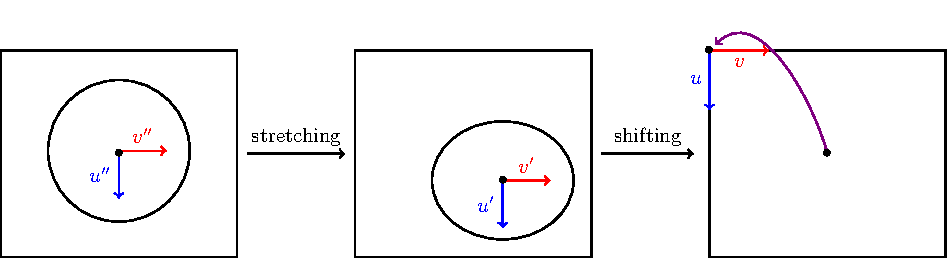
\includegraphics[width=0.9\textwidth]{./fig/tikz/ellipse.pdf}
	\caption{Encompassing ellipse fitting~\cite{scaramuzzacalibration}.}
	\label{fig:ellipse}
  \end{figure}
The intrinsic parameters of the camera specify the image format itself, which is influenced by the focal length, sensor size, and optical center. As there are many mapping
functions that can be used while modeling the lens (their precision is limited by the manufacturing process), Scaramuzza et al.~\cite{scaramuzzacalibration} proposed
fitting a polynomial to find the optimal model for lens calibration. The mapping functions are shown in \reffig{fig:mapping_functions}.
\begin{figure}[H]
  \centering
  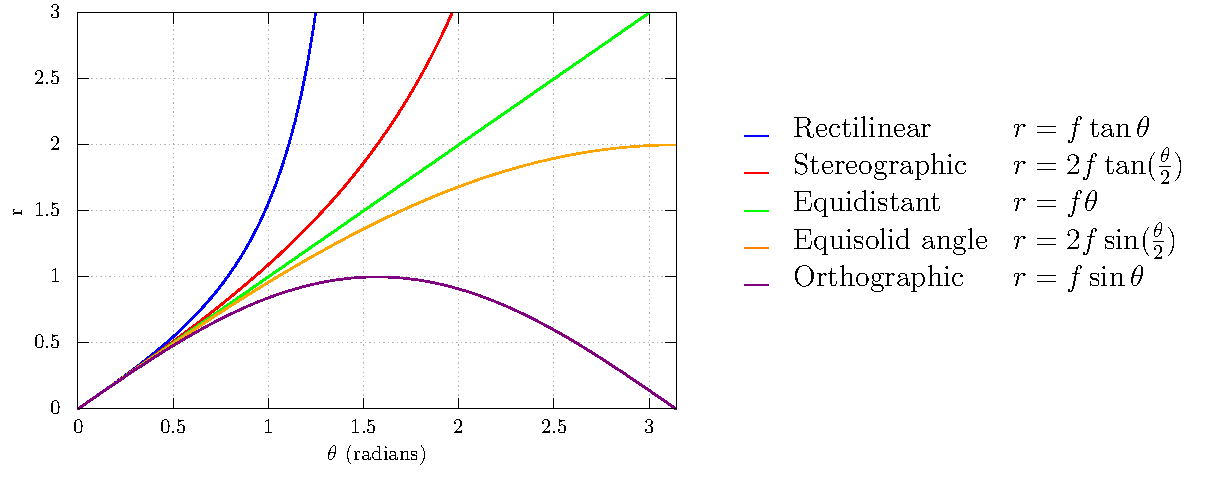
\includegraphics[width=0.9\textwidth]{./fig/tikz/mapping.pdf}
  \caption{Fisheye mapping functions, $f$ is a parameter (focal length).}
  \label{fig:mapping_functions}
\end{figure}

After fitting a polynomial, the image points can be mapped to their corresponding 3D vectors by an equation \ref{eq:intrinsic}.
\begin{equation}
	\lambda \cdot \alpha \cdot
	\begin{bmatrix}
		u' \\
		v' \\
		a_0 + a_1 \rho + \dots + a_{N} \rho^{N} 
	\end{bmatrix}
	= \mathbf{P} \cdot \mathbf{X_w} = %TODO: DOUBLE CHECK X_w is really the world point 
	\begin{bmatrix}
		X_c \\
		Y_c \\
		Z_c
	\end{bmatrix}
	\label{eq:intrinsic}
\end{equation}
where:
\begin{itemize}
\item{$\lambda$ is a scalar factor}
\item{$\alpha$ is a scaling factor that is obtained from \reffig{fig:ellipse} by stretching the ellipse back to a circle and performing
the affine transformation; $\alpha, \lambda > 0$}
\item{$\rho$ is the Euclidean distance of a point from the center; $\rho = \sqrt{u^2 + v^2}$}
\item{$a_0, \dots a_N$ are the polynomial coefficients and $\mathbf{P}$ is 
the perspective projection matrix.}
\end{itemize}

Another relation between a point $\textbf{m}' = \begin{bmatrix} u' & v' \end{bmatrix}^{T}$ in the image plane
and its corresponding point on the sensor plane $\textbf{m} = \begin{bmatrix} u & v \end{bmatrix}^{T}$ can also be written. The coordinates of
$\textbf{m}'$ have the origin at the top left corner of the image, whereas the coordinates of $\textbf{m}$ have the origin in the center of the image.
This can be represented by an affine transformation $\textbf{m}' = \textbf{Am} + \textbf{O}_c$, on \ref{eq:affine}~\cite{URBAN201572}.

\begin{equation}
	\begin{bmatrix}
		u' \\
		v'
	\end{bmatrix}
	= 
	\begin{bmatrix}
		c & d \\
		e & 1
	\end{bmatrix}
	\begin{bmatrix}
		u \\
		v
	\end{bmatrix}
	+
	\begin{bmatrix}
		o_u \\
		o_v
	\end{bmatrix}
\label{eq:affine}
\end{equation}

where matrix $\textbf{A}$ accounts for lens-sensor misalignment, and the vector $\textbf{O}_c$ captures the relation with the center of the distortion. 



% ============= DISTANCE / POSE ESTIMATION ===========

\section{Pose estimation}
% For pose estimation, one can leverage many different approaches, either directly relying on the event data stream itself, or integrating the
% events over time (thus producing a grayscale image or a heatmap), and then estimating the position from the produced image. As we show in \refchap{chap:results}, the number of events
% generated by \ac{LED} sources decreases monotonically with the square of the distance and also decreases with increasing modulation frequency.
% We could then assume that a simple distance predictor could be made by simply fitting a curve to the training dataset consisting of an average
% number of events per blinking period (thus training this predictor for average number of events with respect to distance) and then making the prediction of distance by calculating the average in real time and getting an estimation from the trained predictor.

% This is possible to do in very specific cases where the camera settings and the scene lighting conditions do not change between training measurements
% and the deployment. For example, changing the \texttt{bias-diff-on} or \texttt{bias-diff-off} settings of the camera changes the brightness-change threshold on
% which the camera generates events.
% This changes the number of events that are generated without any information on the distance from the camera, this is similar to changing the exposure
% time on a global shutter camera, which can then give an under- or over-exposed frame.
% It also does not generalize the problem of estimating the position of an arbitrary \ac{UAV} marked with \ac{LED} lights and a camera with previously unspecified
% settings. For a more robust way of estimating the pose of the \ac{UAV} from the camera, we can leverage the following methods.

Pose estimation can be approached in multiple ways using event-based vision. One way of solving the problem is to directly process the
event stream, treating it as a signal
that captures the average number of events that occur in certain areas of the sensor.
Alternatively, events can be accumulated over time to produce a grayscale image
(or a heatmap) that can be analyzed using conventional computer vision techniques for pose estimation.

\subsection{RSSR}

The \ac{RSSR} method provides an approach to estimate the position of an object by measuring the relative ratio of received optical powers from \ac{LED}
markers. This is done by making each of the \ac{LED} markers radiate in their assigned time slot, measuring their optical powers at the time of the
radiation. Jung et al.~\cite{sooyongrssr} demonstrated the \ac{RSSR} method using a configuration where four LED lamps were mounted on the ceiling
with a detector mounted on top of a moving object, parallel to the ceiling.
They have arrived at the equation \refeq{eq:rssr} which could be used to describe the power ratio $RSSR_{1,2}$
\begin{equation}
RSSR_{1,2} = \frac{P_{R1}}{P_{R2}} = \left( \frac{d_2}{d_1} \right)^{n+3}
\label{eq:rssr}
\end{equation}
where $P_{R1}$ and $P_{R2}$ are the received powers of the \ac{LED}s, $d_1$ and $d_2$ are the distances to the \ac{LED}s, and $n$ is the mode number of the radiation lobe (for a Lambertian model $n = 1$).
The \ac{RSSR} pose estimation approach typically consists of a combination of a photo diode, which records the intensity of visible light used for the ratio
calculation, and a camera used to capture visual data~\cite{bai2020highcoveragecameraassisted}.
The method also requires properly calibrated \ac{LED} transmitters, with precisely known emission parameters at a known spatial configuration relative
to the receiver. This then allows for a reliable estimation of the pose.
The method is not used for pose estimation in this thesis due to the lack of time required and the inconclusive results during the analysis of
the measured data (no special calibration of the \ac{LED} transmitters was performed).
It will be explored in future work, where it could be used to improve localization precision, if the method is found to be feasible for the application
of localizing fast moving \ac{UAV}s.

\subsection{Perspective-n-Point}
The \ac{PnP} method has emerged as particularly robust for pose estimation that, unlike \ac{RSSR}, does not rely on signal strength measurements. The method addresses the estimation of the position of an object relative to the camera, having six \ac{DOF}
\begin{itemize}
\item{Rotation - roll, pitch and yaw}
\item{Translation - 3D vector representing the position of the object relative to the camera}
\end{itemize}
This estimation is performed given a set of $n$ known 3D points $\{\mathbf{P}_i\}_{i=1}^n$ on the object and their corresponding 2D projections $\{\mathbf{p}_i\}_{i=1}^n$ in the image plane.
In our application, the UAV has four \ac{LED}-marked arms, where each of them is distinguishable by the camera as a point light source.
However, due to physical limitations, only three \ac{LED}s may be visible at a single point in time, the fourth obstructed by the physical structure of the \ac{UAV} when viewed from the front.
For a case of only 3 image points, the problem becomes the minimal solvable case, called \ac{P3P}, which 
can be formulated as a set of 3D points $\textbf{P}_i \in \mathbb{R}^{3}, i \in \{1, 2, 3\}$ in the world coordinate system, with their corresponding normalized image points
$\textbf{p}_i \in \mathbb{R}^{2}$, $|\textbf{p}_i|=1, i \in \{1, 2, 3\}$. These sets of points are related by a rigid transformation~\cite{Ding_2023_CVPR}
\begin{equation}
d_i \textbf{p}_i = \textbf{R} \textbf{P}_i + \textbf{t}
\label{eq:p3p}
\end{equation}
where $d_i \in \mathbb{R}^+$.
Given the rigid transformation relationship shown in \refeq{eq:p3p}, the \ac{P3P} problem reduces to solving for the rotation matrix 
$\mathbf{R} \in \text{SO}(3)$, translation vector $\mathbf{t} \in \mathbb{R}^3$, and depths $d_i > 0$. 
By exploiting geometric constraints between the 3D points and their 2D projections, the problem can be
reformulated algebraically and solved using various techniques. In our approach, the method proposed by Kneip et al.~\cite{kneip} is used, which
directly finds the rotation and translation with a novel parameterization of the model.
The visualization of the \ac{P3P} problem is shown on \reffig{fig:p3p}.
\begin{figure}[H]
	\centering
	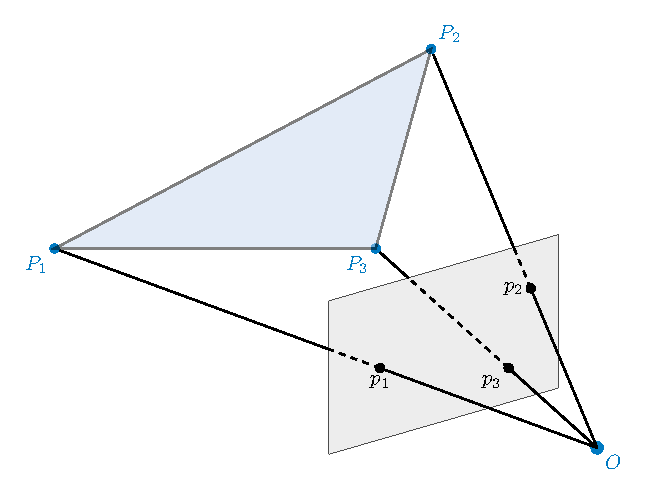
\includegraphics[width=0.75\textwidth]{./fig/tikz/p3p.pdf}
	\caption{P3P problem visualization}
	\label{fig:p3p}
\end{figure}
In our implementation, the average of the estimated pose and distance is computed, thus simplifying the problem of identifying the correct solution from
up to four provided candidates.
If all four \ac{LED}s on the \ac{UAV} are detected, a general \ac{PnP} solution is calculated using the \ac{RANSAC} method.
This yields only one solution, so the estimated distance is simply the distance from the camera to the geometric center of the \ac{UAV}.